\chapter{Introduction to FDTD Methods}\label{ch:FDTD}

\begin{flushright}{\it
``Since Newton, mankind has come to realize that the laws of physics\\
are always expressed in the language of differential equations.''\\
- Steven Strogatz} %\\
%\SWcomment[(https://youtu.be/O85OWBJ2ayo?t=44)]
\end{flushright}
%
\vspace{2em}
This chapter introduces some important concepts needed to understand the physical models presented later on in this document. 
By means of a simple mass-spring system and the 1D wave equation, the notation and terminology used throughout this document will be explained. 
Before diving into the mathematics, let us go over some useful terminology.

\section{Differential Equations}
Differential equations are used to describe the motion of dynamic systems including vibrations in musical instruments. In this work, these equations are used, among others, to describe the movement of a string, an instrument body and the air pressure in an acoustic tube.

A characteristic feature of these equations is that, rather than an absolute value or \textit{state} of a system, the time derivative of its state -- its velocity -- or the second time derivative -- its acceleration -- is described. From this, the absolute state of the system can then be computed.
%
This state is usually described by the variable $u$ which is (nearly) always a function of time, i.e., $u=u(t)$. If the system is distributed in space, $u$ also becomes a function of space, i.e., $u = u(x,t)$, or with two spatial dimensions, $u = u(x,y,t)$, etc. Though this work only describes systems of up to two spatial dimensions, one can easily extend to three dimensions \cite{Hamilton2016} and potentially higher-dimensional systems \cite{Bustamante2017}\todo{maybe not such a relevant reference..}! See Section \ref{sec:dimensions} for more information on this.
% one could potentially extend to systems of infinite spatial dimensions evolving over time!

If $u$ is univariate, and only a function of time, the differential equation that describes the motion of this system is called an \textit{ordinary differential equation} (ODE). Various ways to describe the second derivative in time of $u$, or the acceleration of $u$ are
%
\begin{equation}\nonumber
    \begin{aligned}
        \frac{d^2 u}{d t^2} & \quad \text{(Leibniz's notation)},\\
        \ddot u\ \  &\quad \text{(Newton's notation)},\\[3pt]
        D_t^2 u& \quad \text{(Euler's notation)}.
    \end{aligned}
\end{equation}
%
Leibniz' notation could be considered the most standard notation but is not necessarily compact. Newton's notation on the other hand allows for an ultra compact notation using a dot above the function to denote a derivative. However, this notation can only be used for univariate functions which it will be used for in this document. Finally, Euler's notation uses an operator which can be applied to a function and indicates a derivative.  
 
If $u$ is also a function of at least one spatial dimension, the equation of motion is a called a \textit{partial differential equation} (PDE).
The literature uses different types of notation for taking (continuous-time) partial derivatives. Applied to a state variable $u$ these can look like 
\begin{equation}\nonumber
    \begin{aligned}
        \frac{\partial^2 u}{\partial t^2} & \quad \text{(Leibniz's notation)}\\
        u_{tt}\:\,& \quad \text{(subscript notation)}\\[3pt]
        \ptt u\: & \quad \text{(Euler's notation)}
    \end{aligned}
\end{equation}
% 
%
% \begin{equation}\nonumber
%     \begin{aligned}
%         \frac{\partial^2 u}{\partial t^2}, \quad
%         u_{tt},\quad
%         \ptt u
%     \end{aligned}
% \end{equation}
%
where the subscript notation could be seen as the partial derivative counterpart to Newton's notation due to its compactness. In the remainder of this document, the operator notation will be used, due to their similarity to the discrete operators (introduced shortly) and as it allows for creation of bigger operators for more compactness when working with multiple (connected) systems (see e.g. Chapter \ref{ch:tromba}).

Often-used partial derivatives and their meanings \todo{maybe not yet as this is super general still} are shown below

\begin{minipage}[c]{0.49\textwidth}
    \begin{align*}
        \ptt u &\quad \text{(acceleration)}\\
        \pt u &\quad \text{(velocity)}
    \end{align*}
\end{minipage}
\begin{minipage}[c]{0.49\textwidth}
    \begin{align*}
    \pxx u &\quad \text{(curvature)}\\
    \px u &\quad \text{(slope)}
    \end{align*}
\end{minipage}

\subsection{Dimensions and Degrees of Freedom}\label{sec:dimensions}
All objects in the physical world are 3-dimensional (3D) as they have a non-zero width, length and depth. Moreover, these objects can move in these three dimensions and thus have three translational \textit{degrees of freedom (DoF)} \SWcomment[(the three rotational DoF are ignored here)]. 
To reduce the complexity of the model as well as computational complexity, simplifications can be made to reduce both the dimensionality of the spatial distribution of a physical object as well as that of the translational DoF. 

Generally, the spatial distribution of an object can be simplified if one (or more) of the dimensions is orders of magnitude smaller than the others. A guitar string, for instance, has much greater length than its width or depth and can therefore be reduced to a one-dimensional (1D) system. If a 3D description were to be kept, the relative displacement between two locations on one cross-section along the length of the string would be taken into account. One could imagine that this displacement will always be orders of magnitude smaller than the relative displacement of two points along the string length and is thus negligible. Similarly, the thickness of a drum membrane is much smaller than its length and width and can therefore be simplified to a two-dimensional (2D) system. 

The translational DoF\todo{check whether this needs to be per point along a system}, on the other hand, describe now many ``coordinates'' a state variable includes. 
In much of the literature on FDTD methods in the field of musical acoustics, the state variable only has one coordinate. In most string models, for example, only the transverse displacement in one polarisation is considered (see Chapter \ref{ch:stiffString}) and the other polarisation as well as the longitudinal motion of the string is ignored. In other words, every point along the string can only move up and down, not side-to-side and not forward and back. Although this greatly simplifies the system at hand and reduces computational complexity, this is not what happens in reality, and non-linear effects such as phantom partials and pitch glides due to tension modulation are not present in the simplified model. 

Work has been done on strings with dual polarisation by Desvages \cite{Desvages2018} and Desvages and Bilbao \cite{Desvages2016} using FDTD methods. Models including longitudinal string vibration, where the longitudinal and transversal displacements are couples can be found in \cite{theBible,Bilbao2009spring}.
In \cite{Villeneuve2019}, Villeneuve and Leonard present a mass-spring network where the state of every individual mass has three translational DoF. Due to these additional DoF, these networks would capture the aforementioned effects, but greatly increase the computational complexity of the models. 

Although the dimensionality reduction ignoring some of the physical processes, surprisingly realistic sounding models can be made despite these simplifications. Due to computational considerations, all models used in this work thus only have 1 translational DoF.

\subsubsection{Notation}
When describing the state of a system, the spatial dimensions it is distributed over appears in the argument of the state variable, whereas the translational DoF determines the amount of coordinates of the state variable describes. For example, the state of a 2D system, with 1 translational DoF is written as $u(x,y,t)$. A 1D system with 3 translational DoF can be written as $\mathbf{u}(x,t)$ where $\mathbf{u}$ is a vector containing the coordinates for all three translational DoF.  

% What this means for the notation introduced in the previous section is  the amount of arguments for the state variable. As all systems (in this context) have one temporal dimension, the state of a 1D system -- such as a string -- is described using $u(x,t)$, a 2D system -- such as a membrane -- is described using $u(x,y,t)$, and the state of a simple zero-dimensional (0D) mass-spring system as $u(t)$.

\subsection{Domains}\label{sec:domains}
When describing physical systems using state variables, \textit{domains} over which they are defined need to be provided. This means that for the state of a 1D system $u = u(x,t)$, ranges of definition must be given for $x$ and $t$. Usually, time $t\geq 0$, meaning that the system is defined for non-negative time. For the spatial dimension, we may define a finite domain $\D$ over which $x$ is defined, which is written as $x\in \D$. For analysis purposes, infinite domains ($\D = \mathbb{R} = (-\infty, \infty)$) or semi-infinite domains ($\D = \mathbb{R}^+ = [0, \infty)$) may be used, but for implementation purposes, a finite domain needs to be established.

\section{Discretisation using FDTD methods}
Differential equations are powerful tools that describe the motion of physical systems. Despite this, only few of these have a closed-form \SWcomment[or analytical] solution (such as the simpler ones that will be presented in this chapter). More complex systems require methods that do not perfectly solve, but rather \textit{approximate} the solutions to these equations. Finite-difference time-domain (FDTD) are considered one of the
in terms of generality and flexibility... 

Unless denoted otherwise, the equations and theory used in this chapter has been taken from \cite{theBible}.

\SWcomment[It is important to note that a discrete FD scheme is an \textit{approximation} to a continuous PDE, not a sampled version of it. This means that the resulting schemes are rarely an exact solution to the original continuous equation.]

These methods essentially subdivide a continuous differential equation into discrete points in time and space, a process called \textit{discretisation}. Once an ODE or PDE is discretised using these methods it is now called a \textit{finite-difference (FD) scheme} which approximates the original differential equation. In the following, for generality and ease of explanation, a 1D system will be used.

\begin{figure}[h]
    \centering
    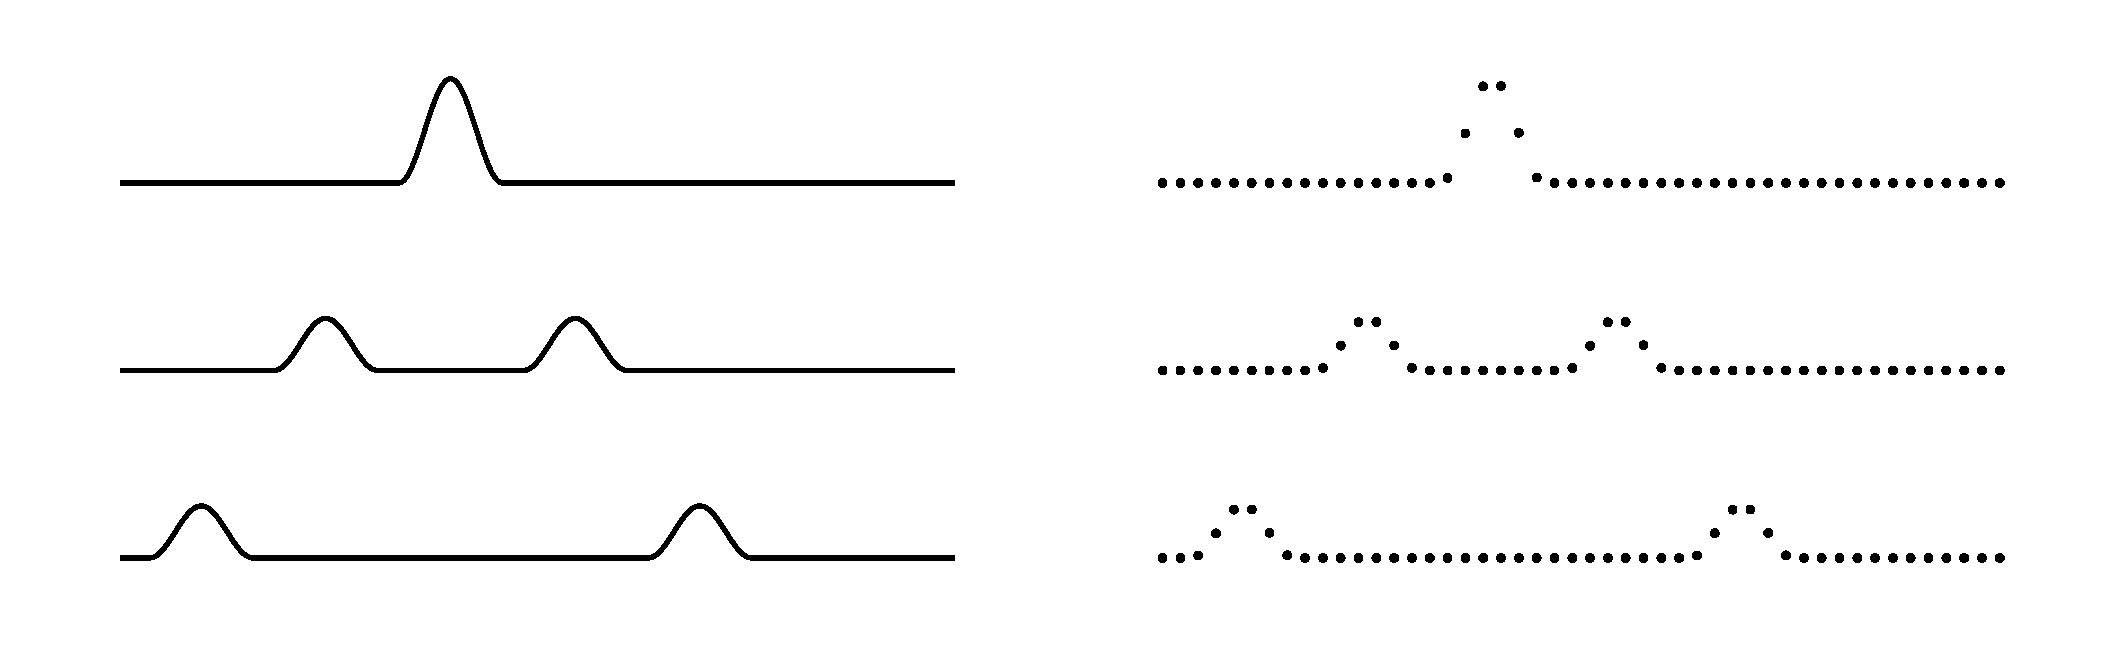
\includegraphics[width=\textwidth]{figures/fdtd/gridFigure.eps}
    \caption{\label{fig:discretisation} A continuous PDE is discretised... }
\end{figure}\todo{Figure and caption are not done yet}

\subsection{Grid Functions \todo{FULL DOC SWEEP: check capitalisation of headings throughout document}} \label{sec:gridFunctions}
We start by defining a discrete \textit{grid} over time and space which we will use to approximate our continuous equations \todo{grid figure}. A system described by state $u = u(x,t)$ defined over time $t$ and one spatial dimension $x$, can be discretised to a \textit{grid function} $u_l^n$. Here, integers $l$ and superscript $n$ describe the spatial and temporal indices respectively and arise from the discretisation of the continuous variables $x$ and $t$ according to $x=lh$ and $t=nk$. The spatial step $h$, also called the \textit{grid spacing} describes the distance (in m) between two neighbouring \textit{grid points} and the temporal step $k$, or \textit{time step} is the time (in s) between two consecutive temporal indices. The latter can be calculated $k=1/\fs$ for a sample rate $\fs$ (in Hz). In many audio applications $\fs = 44100$ Hz which will be used in this work (unless denoted otherwise).

% \subsubsection{Discrete Domains}
As mentioned in Section \ref{sec:domains}, a 1D system needs to be defined over a temporal and one spatial domain.
In discrete time, the temporal domain $t \geq 0$ is discretised to $n \in \mathbb{N}^0$.\footnote{In this work, $\mathbb{N}^0$ is used to denote the set of non-negative integers ($\mathbb{N}^0 = 0, 1, 2, 
\hdots$).} 
The spatial domain $\D$ can be subdivided into $N$ equal sections, or intervals, of length $h$ (see Figure \ref{fig:gridExp}). The grid points describing the state of the system are placed between and around these intervals. The spatial range of interest then becomes $l\in \{0, \hdots, N\}$ and the total number of grid points is $N+1$, one more than the number of intervals. 

%The grid points interact with their neighbouring grid points according to the model at hand.

% At the ends of each section there needs to be grid point describing the discrete state of the system at each sections needs to be 

%Consider a (continuous-time) system, $u = u(x,t)$ defined over time $t\geq 0$ and space $x\in \D$ with domain $\D = [0, L]$. Time can be subdivided in 

\todo{this might be unnecessary, but I thought that it might be nice to have this in an equation for clarity} To summarise, for a 1D system
\begin{equation*}
    u(x,t) \approx u_l^n \quad \text{with} \quad x=lh \quad \text{and} \quad t = nk,
\end{equation*}
\begin{equation*}
    l\in\{0, \hdots, N\}\qaq n \in \mathbb{N}^0.
\end{equation*}

\begin{figure}[h]
    \centering
    % \subfloat[If $N=5$ there are 5 sections of length $h$ and 6 grid points describing the state of the system ($l=\{0, \hdots, 5\}$).\label{fig:gridExp1}]{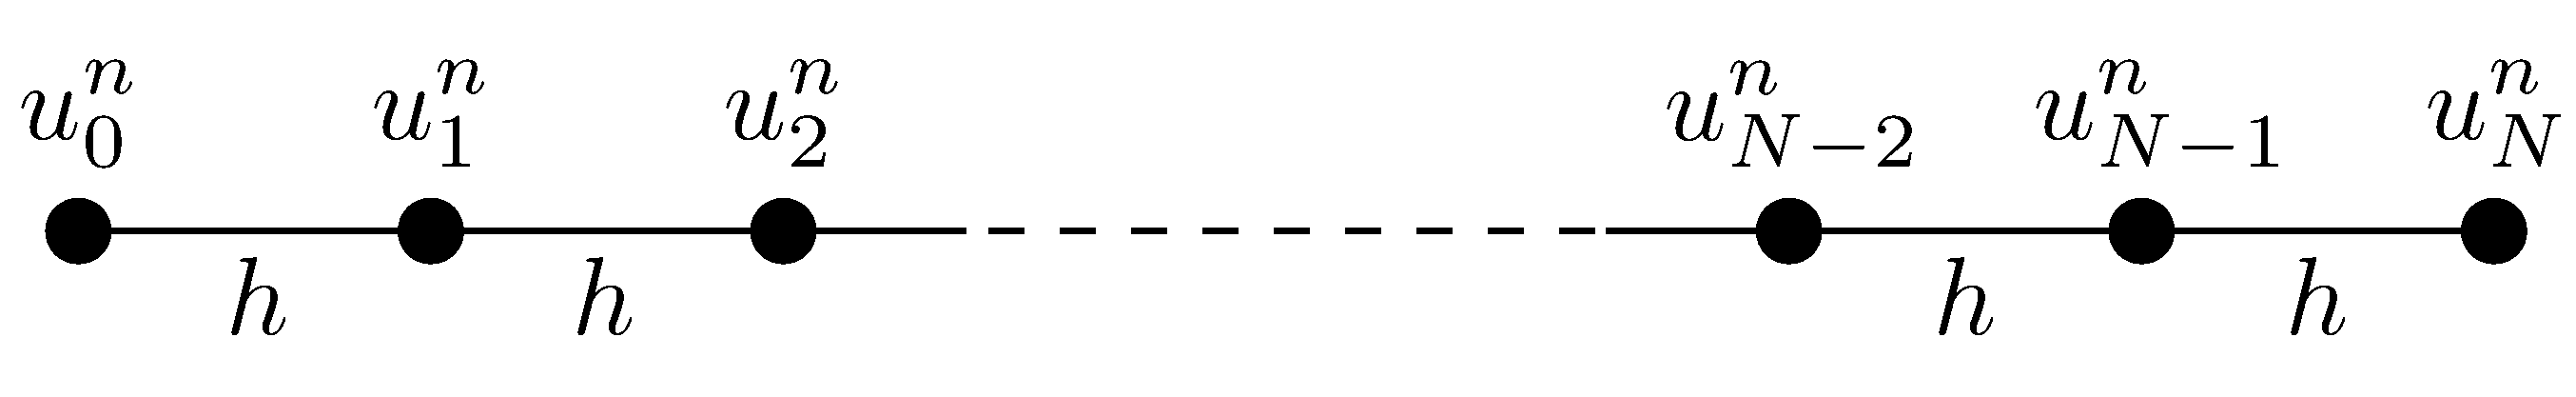
\includegraphics[width=0.45\textwidth]{figures/fdtd/gridExplanation.pdf}}\hspace{0.06\textwidth}
    % \subfloat[If $N$ is large (as is usually the case), The 1D system is divided into $N$ sections of length $h$ and $l=\{0, \hdots, N\}$.\label{fig:gridExp2}]{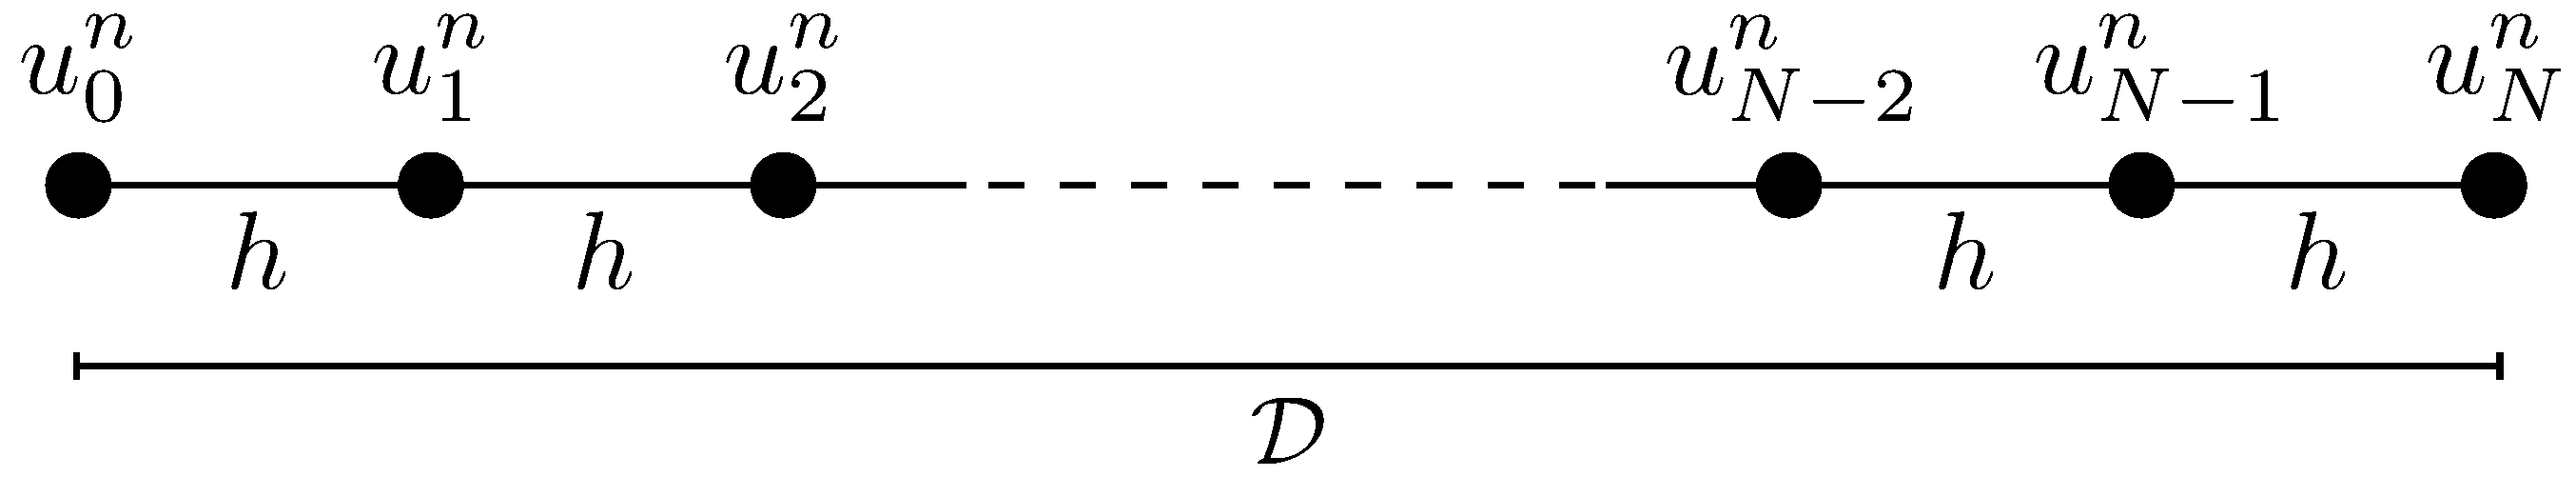
\includegraphics[width=0.45\textwidth]{figures/fdtd/gridExplanation2.pdf}}
    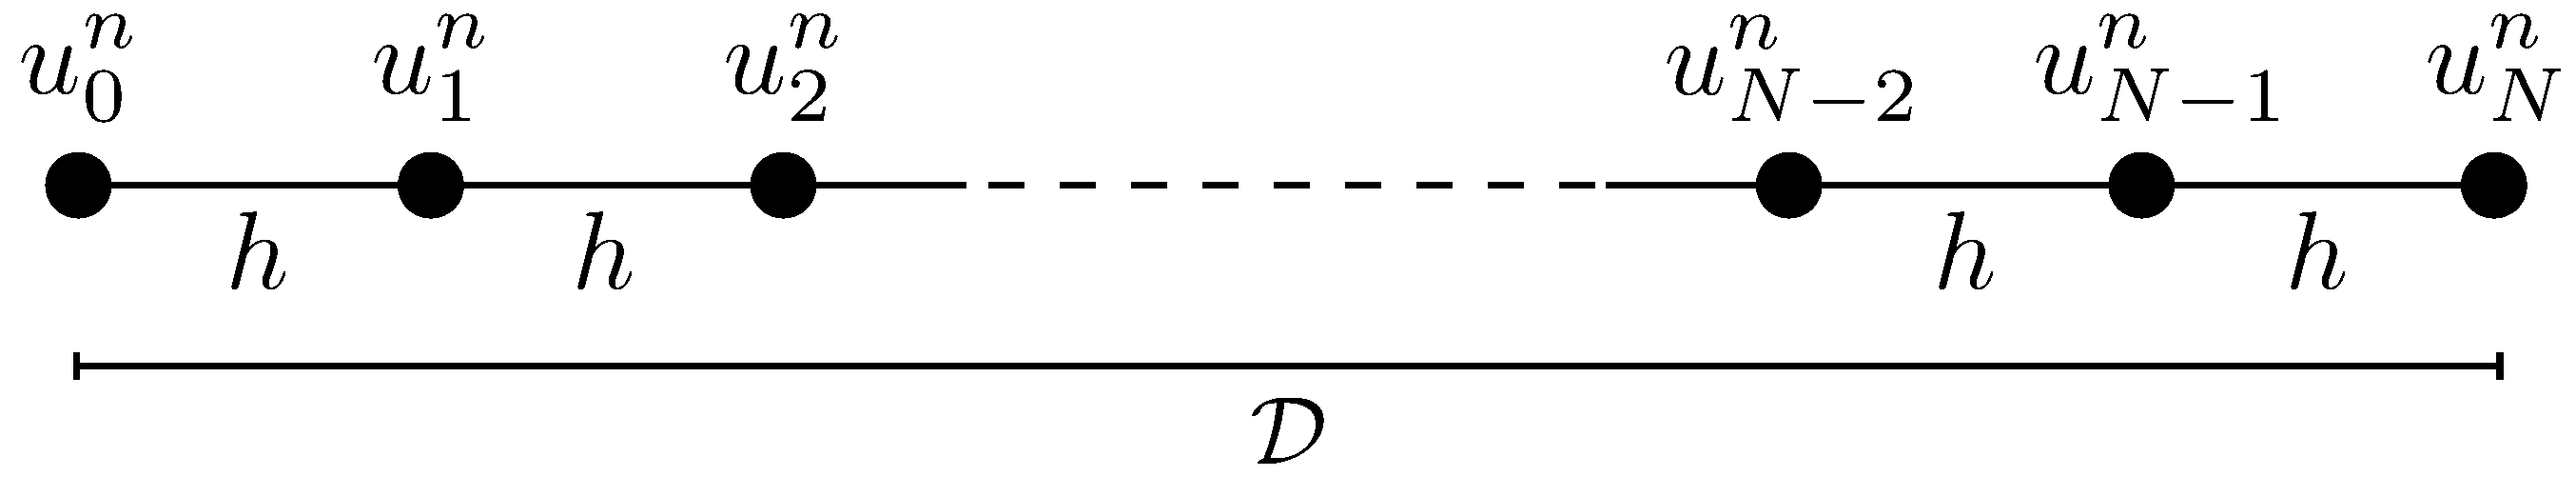
\includegraphics[width=0.75\textwidth]{figures/fdtd/gridExplanation2.pdf}
    \caption{When a 1D system $u(x,t)$ with $x\in \D$ is discretised to a grid function $\uln$, the spatial domain $\D$ is divided into $N$ intervals of length $h$ and spatial range of interest $l=\{0, \hdots, N\}$.\label{fig:gridExp}}
\end{figure}

\subsection{Finite-Difference Operators}\label{sec:FDoperators}
Now that the state variable has a discrete counterpart, this leaves the derivatives to be discretised, or approximated. We start by introducing shift operators that can be applied to a grid function and `shifts' its indexing, either temporally or spatially. Forward and backward shifts in time, together with the identity operation are
% 
\begin{equation}\label{eq:temporalShifts}
    e_{t+}\uln = u_l^{n+1},\quad e_{t-}\uln = u_l^{n-1}, \quad \text{and} \quad 1\uln = \uln.
\end{equation}
%
Similarly, forward and backward shifts in space are
%
\begin{equation}\label{eq:spatialShifts}
    e_{x+}\uln = u_{l+1}^n,\quad \text{and}\quad e_{x-}\uln = u_{l-1}^n.
\end{equation}
%
\todo{many figures for shift and FD operators}These shift operators are rarely used in isolation, though they do appear in energy analysis techniques detailed in Section \ref{sec:energyAnalysis}. The operators do, however, form the basis of commonly used \textit{finite-difference (FD) operators}. The first-order derivative in time can be discretised three different ways. The forward, backward and centred \todo{FULL DOC SWEEP: check centred instead of centered} difference operators are
%
\todo{these spacings are different in overleaf...}
\begin{subnumcases}{\pt \approxeq\label{eq:discFirstTime}}
        \dtp &$\!\!\!\!\!\!\!\!\!\!\triangleq \frac{1}{k}\left(e_{t+} - 1\right),$\label{eq:forwardTimeOperator}\\
        \dtm &$\!\!\!\!\!\!\!\!\!\!\triangleq \frac{1}{k}\left(1 - e_{t-}\right),$\label{eq:backwardTimeOperator}\\
        \dtd &$\!\!\!\!\!\!\!\!\!\!\triangleq \frac{1}{2k}\left(e_{t+} - e_{t-}\right),$\label{eq:centredTimeOperator}
\end{subnumcases}
where ``$\triangleq$'' means ``equal to by definition''. These operators can then be applied to grid function $\uln$ to get
\begin{subnumcases}{\pt u \approxeq\label{eq:discFirstTimeU}}
    \dtp \uln &$\!\!\!\!\!\!\!\!\!\! = \frac{1}{k}\left(u_l^{n+1} - \uln\right),$\label{eq:forwardTimeOperatorU}\\
    \dtm \uln &$\!\!\!\!\!\!\!\!\!\! = \frac{1}{k}\left(\uln - u_l^{n-1}\right),$\label{eq:backwardTimeOperatorU}\\
    \dtd \uln &$\!\!\!\!\!\!\!\!\!\! = \frac{1}{2k}\left(u_l^{n+1} - u_l^{n-1}\right),$\label{eq:centredTimeOperatorU}
\end{subnumcases}
and all approximate the first-order time derivative of $u$. Note that the centred difference has a division by $2k$ as the time difference between $n+1$ and $n-1$ is, indeed, twice the time step. 

\todo{figure here visualising operators (with reference to grid figure)}
Similar operators exist for a first-order derivative in space, where the forward, backward and centred difference are
\begin{subnumcases}{\px \approxeq\label{eq:discFirstSpace}}
    \dxp &$\!\!\!\!\!\!\!\!\!\!\triangleq \frac{1}{h}\left(e_{x+} - 1\right),$\label{eq:forwardSpaceOperator}\\
    \dxm &$\!\!\!\!\!\!\!\!\!\!\triangleq \frac{1}{h}\left(1 - e_{x-}\right),$\label{eq:backwardSpaceOperator}\\
    \dxd &$\!\!\!\!\!\!\!\!\!\!\triangleq \frac{1}{2h}\left(e_{x+} - e_{x-}\right),$\label{eq:centredSpaceOperator}
\end{subnumcases}
and when applied to $\uln$ are
\begin{subnumcases}{\px u \approxeq\label{eq:discFirstSpace}}
    \dxp \uln&$\!\!\!\!\!\!\!\!\!\!= \frac{1}{h}\left(u_{l+1}^n- \uln\right),$\\
    \dxm \uln&$\!\!\!\!\!\!\!\!\!\!= \frac{1}{h}\left(\uln - u_{l-1}^n\right),$\\
    \dxd \uln&$\!\!\!\!\!\!\!\!\!\!= \frac{1}{2h}\left(u_{l+1}^n - u_{l-1}^n\right).$\label{eq:centredSpaceOperatorU}
\end{subnumcases}
Higher order differences can be approximated through a composition of first-order difference operators. The second-order difference in time may be approximated using
\begin{equation}\label{eq:discSecondTime}
    \ptt \approxeq \dtp\dtm = \dtt \triangleq \frac{1}{k^2}\left(e_{t+}-2+e_{t-}\right),
\end{equation}
where ``$2$'' is the identity operator applied twice. This can similarly be done for the second-order difference in space
\begin{equation}\label{eq:discSecondSpace}
    \pxx \approxeq \dxp\dxm = \dxx \triangleq \frac{1}{h^2}\left(e_{x+}-2+e_{x-}\right),
\end{equation}
both of which can be applied to a grid function $\uln$ in a similar fashion.
Further information on combining operators can be found in Section \ref{sec:combiningOperators}.

Also useful \todo{in energy analysis, interleaved grids, etc.} are averaging operators, all of which approximate the identity operation. The temporal forward, backward and centred averaging operators are
\begin{subnumcases}{1 \approxeq \label{eq:averagingTime}}
    \mtp & $\!\!\!\!\!\!\!\!\!\!\triangleq \frac{1}{2}\left(e_{t+} + 1\right),$\label{eq:forwardAvgTime}\\
    \mtm & $\!\!\!\!\!\!\!\!\!\!\triangleq \frac{1}{2}\left(1 + e_{t-}\right),$\label{eq:backwardAvgTime}\\
    \mtd & $\!\!\!\!\!\!\!\!\!\!\triangleq \frac{1}{2}\left(e_{t+} + e_{t-}\right).$\label{eq:centredAvgTime}
\end{subnumcases}
Notice how these definitions are different than the difference operators in \eqref{eq:discFirstTime}: the terms in the parentheses are added rather than subtracted, and rather than a division by the time step $k$ there is a division by $2$. Finally, the centred averaging operator does not have an extra division by $2$ as in \eqref{eq:centredTimeOperator}.
Applied to $\uln$, Eqs. \eqref{eq:averagingTime} become
\begin{subnumcases}{\uln \approxeq \label{eq:averagingTimeU}}
    \mtp \uln & $\!\!\!\!\!\!\!\!\!\!= \frac{1}{2}\left(u_l^{n+1}+ \uln\right),$\label{eq:forwardAvggTimeU}\\
    \mtm \uln & $\!\!\!\!\!\!\!\!\!\!= \frac{1}{2}\left(\uln + u_l^{n-1}\right),$\label{eq:backwardAvggTimeU}\\
    \mtd \uln & $\!\!\!\!\!\!\!\!\!\!= \frac{1}{2}\left(u_l^{n+1} + u_l^{n-1}\right).$\label{eq:centredAvggTimeU}
\end{subnumcases}
%
Similarly, spatial averaging operators are
\begin{subnumcases}{1 \approxeq \label{eq:averagingSpace}}
    \mxp & $\!\!\!\!\!\!\!\!\!\!\triangleq \frac{1}{2}\left(e_{x+} + 1\right),$\label{eq:forwardAvgSpace}\\
    \mxm & $\!\!\!\!\!\!\!\!\!\!\triangleq \frac{1}{2}\left(1 + e_{x-}\right),$\label{eq:backwardAvgSpace}\\
    \mxd & $\!\!\!\!\!\!\!\!\!\!\triangleq \frac{1}{2}\left(e_{x+} + e_{x-}\right),$\label{eq:centredAvgSpace}
\end{subnumcases}
and when applied to $\uln$
\begin{subnumcases}{\uln \approxeq \label{eq:averagingSpaceU}}
    \mxp \uln & $\!\!\!\!\!\!\!\!\!\!= \frac{1}{2}\left(u_{l+1}^n+ \uln\right),$\label{eq:forwardAvgSpaceU}\\
    \mxm \uln & $\!\!\!\!\!\!\!\!\!\!= \frac{1}{2}\left(\uln + u_{l-1}^n\right),$\label{eq:backwardAvgSpaceU}\\
    \mxd \uln & $\!\!\!\!\!\!\!\!\!\!= \frac{1}{2}\left(u_{l+1}^n + u_{l-1}^n\right).$\label{eq:centredAvgSpaceU}
\end{subnumcases}
Finally, using forward and backward averaging operators, second-order temporal and spatial averaging operators can be created according to
\begin{equation}
    1 \approxeq \mtt = \mtp\mtm \triangleq \frac{1}{4}\left(e_{t+}+2+e_{t-}\right),
\end{equation}
and
\begin{equation}
    1 \approxeq \mxx = \mxp\mxm \triangleq \frac{1}{4}\left(e_{x+}+2+e_{x-}\right).
\end{equation}

Operators and derivatives in 2D will be discussed in Chapter \ref{ch:2Dsyst}.


\subsubsection{Accuracy}
As FDTD methods approximate continuous systems, the resulting solution is rarely 100\% accurate. To determine the accuracy of the FD operators above, one can perform a Taylor series analysis. The Taylor series is an infinite sum and its expansion of a function $f$ about a point $a$ is defined as
\begin{equation}
    f(x) = \sum_{n=0}^{\infty} \frac{(x-a)^n}{n!}f^{(n)}(a)
\end{equation}
where superscript $(n)$ denotes the $n$\th derivative of $f$ with respect to $x$. The analysis will be performed on the temporal operators in this section, but also apply to the spatial operators presented.

Using continuous function $u=u(t)$ and following Bilbao's ``slight abuse of notation'' in \cite{theBible}, one may apply FD operators to continuous functions according to 
\begin{equation}\label{eq:forwardTimeCont}
    \dtp u(t) = \frac{u(t+k) - u(t)}{k}\ .
\end{equation}
%
Assuming that $u$ is infinitely differentiable, $u(t+k)$, i.e., $u$ at the next time step (but in continuous time), can be approximated using a Taylor series expansion of $u$ about $t$ according to
\begin{equation}\label{eq:taylorStartForward}
    u(t+k) = u(t) + k \dot u + \frac{k^2}{2} \ddot u + \frac{k^3}{6} \dot{\ddot{u}} + \O(k^4).
\end{equation}
Here, (following Newton's notation) the dot describes a single temporal derivative and $\O$ includes additional terms in the expansion. The power of $k$ in the argument of $\O$ describes the order of accuracy, the higher the power of $k$ the more accurate the approximation. Equation \eqref{eq:taylorStartForward} can be rewritten to 
\begin{align}
    \frac{u(t+k) - u(t)}{k} &= \dot u + \frac{k}{2} \ddot u +\frac{k^2}{6} \dot{\ddot{u}} + \O(k^3),\nonumber\\
    % \dot u &= \frac{u(t+k) - u(t)}{k} + \O(k),
    \dtp u(t) &= \dot u + \O(k),
\end{align}
which says that the forward difference operator approximates the continuous first order derivative with an additional error term.
As the power of $k$ in $\O$'s argument is $1$, it can be concluded that the forward operator is first-order accurate. One can also observe that, as expected, the error gets smaller as the time step $k$ gets smaller and indicates that higher sample rates result in more accurate simulations (through $k=1/\fs$).

We can arrive at a similar result for the backward operator. Applying Eq. \eqref{eq:backwardTimeOperator} to $u$ yields
\begin{equation}
    \dtm u(t) = \frac{u(t) - u(t-k)}{k}
\end{equation}
and performing a Taylor series expansion of $u$ about $t$ yields
\begin{align}
    u(t-k) &= u(t) + (-k) \dot u + \frac{(-k)^2}{2} \ddot u +\frac{(-k)^3}{6}\dot{\ddot{u}} + \O(k^4),\label{eq:taylorStartBackward}\\
    \frac{u(t-k) - u(t)}{k} &= -\dot u + \frac{k}{2} \ddot u - \frac{k^2}{6}\dot{\ddot{u}} + \O(k^3),\nonumber\\
    % \dot u &= \frac{u(t) - u(t-k)}{k} + \O(k).
    \dtm u(t) &= \dot u + \O(k).
\end{align}
Notice that the sign of $\O$ does not matter.

Applying the centred operator in Eq. \eqref{eq:centredTimeOperator} to $u$ yields
\begin{equation}
    \dtd u(t) = \frac{u(t+k) - u(t-k)}{2k},
\end{equation}
indicating that to find the order of accuracy for this operator, both Eqs. \eqref{eq:taylorStartForward} and \eqref{eq:taylorStartBackward} are needed. Subtracting these and filling in their definitions yields
\begin{align}
    u(t+k) - u(t-k) &= 2k\dot u - \frac{2k^3}{6}\dot{\ddot{u}} + 2\O(k^5),\nonumber\\
    \frac{u(t+k) - u(t-k)}{2k} &= \dot u + \O(k^2),\nonumber\\
    \dtd u(t) &= \dot u + \O(k^2),
\end{align}
and shows that the centred difference operator is second-order accurate. 

As a first-order derivative indicates the \textit{slope} of a function, the differences in accuracy between the above operators can be visualised as in Figure \ref{fig:taylor}. It can be observed that the derivative approximation of the centred operator much more closely matches the the true derivative of $u$ at $t$.

\begin{figure}[h]
    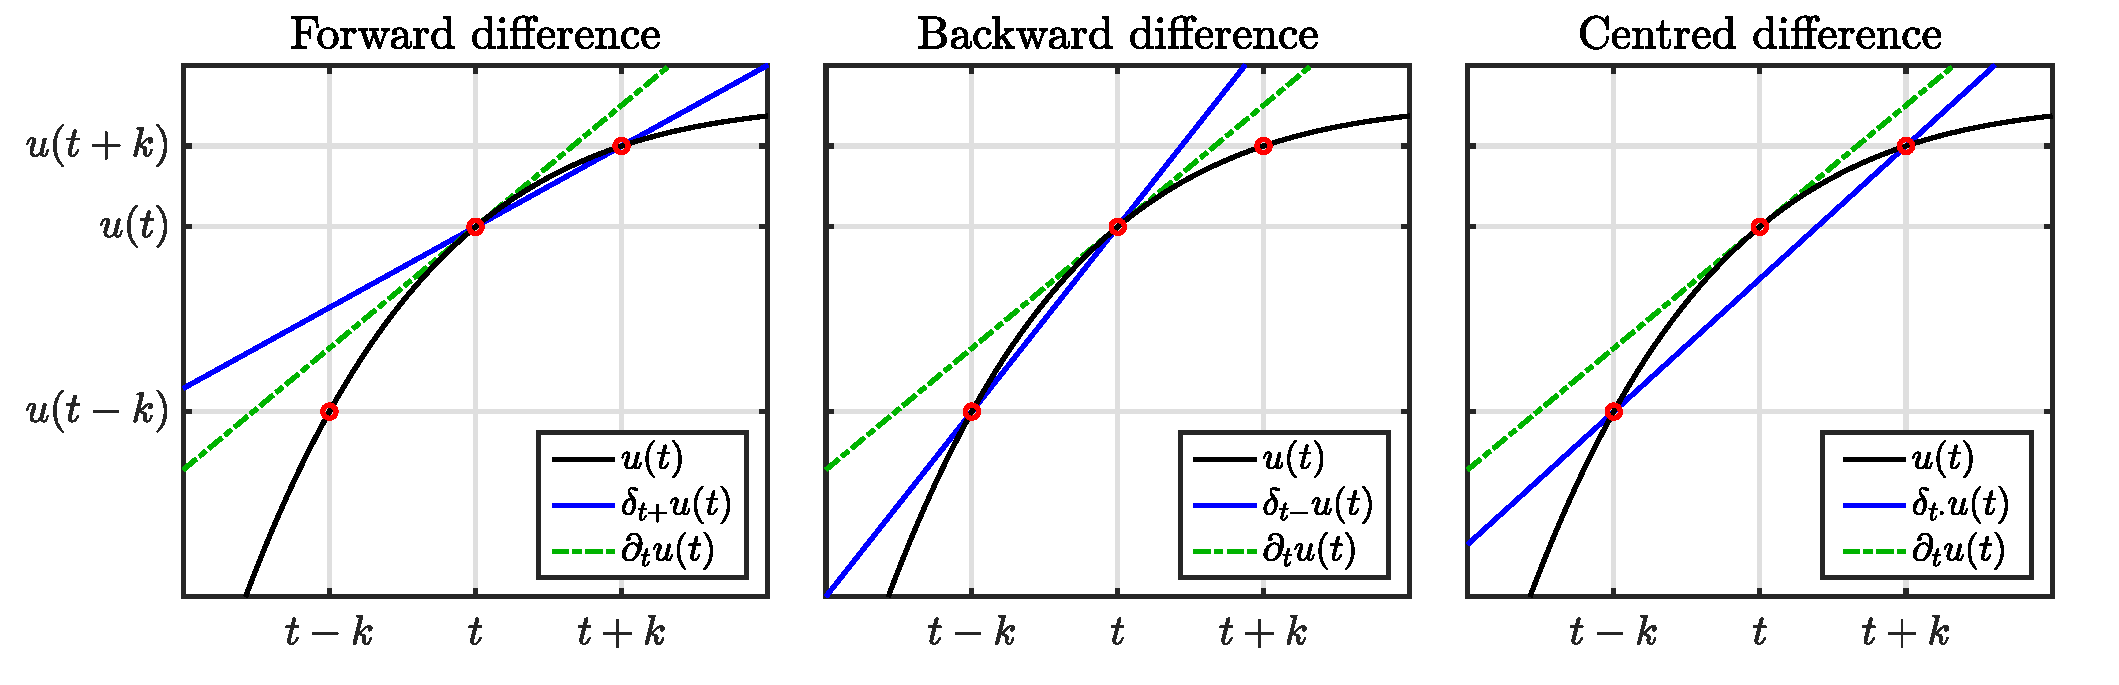
\includegraphics[width=\textwidth]{figures/fdtd/taylor.eps}
    \caption{\label{fig:taylor} The accuracy of the forward, backward and centred difference operators in \eqref{eq:discFirstTime} visualised. One can observe that the centred difference operator much more closely approximates the derivative, or the slope, of $u$ at $t$ than the forward and backward difference operators.}
\end{figure}

Higher-order differences, such as the second-order difference in time operator in Eq. \eqref{eq:discSecondTime} can also be applied to $u(t)$ to get
\begin{equation}
    \dtt u(t) =  \frac{u(t+k) - 2u(t) + u(t-k)}{k^2},
\end{equation}
and be proven to be second-order accurate by adding Eqs. \eqref{eq:taylorStartForward} and \eqref{eq:taylorStartBackward}:
\begin{align}
    u(t+k) + u(t-k) &= 2 u(t) + k^2 \ddot u + \O(k^4),\nonumber\\
    \frac{u(t+k) -2 u(t) + u(t-k)}{k^2} &= \ddot u + \O(k^2),\nonumber\\
    \dtt u(t) &= \ddot u + \O(k^2).
\end{align}

The accuracy of averaging operators can also be found and follow a similar pattern. 
\begin{equation}
    \begin{gathered}
    \mtp u(t) = u(t) + \O(k),\quad \mtm u(t)= u(t) + \O(k),\\
    \mtd u(t)= u(t) + \O(k), \quad \mtt u(t)= u(t) + \O(k^2).
    \end{gathered}
\end{equation}

\subsection{Identities}
For working with FD schemes, either for implementation or analysis, it can be extremely useful to rewrite the operators presented above to equivalent versions of themselves. These are called identities and for future reference, some useful ones are listed below
\begin{subequations}
    \begin{align}
        \dtt &= \frac{2}{k}\left(\dtd- \dtm\right)\label{eq:identity1}\\
        \dtd &= \dtp\mtm = \dtm\mtp\label{eq:identity2}\\
        \mtp &= \frac{k}{2}\dtp + 1\label{eq:identity3}
    \end{align}
\end{subequations}
\todo{see whether the negative version of identity \eqref{eq:identity3} is also used later on}
That these equalities hold can easily be proven by expanding the operators defined in Section \ref{sec:FDoperators}. Naturally, these identities also hold for spatial operators by simply substituting the `$t$' subscripts for `$x$'. 

\section{%Intro to ODEs: 
The Mass-Spring System}\label{sec:massSpringSystem}
Though a complete physical modelling field on its own (see Chapter \ref{ch:physMod}), mass-spring systems are also sound-generating systems themselves and lend themselves well to illustrating and explaining FDTD methods in practice. Starting with the continuous-time ODE, this section continues to discretise it to an FD scheme using the operators described in Section \ref{sec:FDoperators}. Finally, the scheme is rewritten to an update equation that can be implemented and the output of the system is shown. 

\subsection{Continuous-time}\label{sec:massSpringCont}
Using dots to indicate a temporal derivative, the ODE of a simple mass-spring system is defined as
\begin{equation}\label{eq:massSpringPDE}
    M\ddot u = -Ku,
\end{equation}
where $u = u(t)$ is the distance from the equilibrium position (in m), $M$ \SWcomment[$>0$] is the mass of the mass (in kg) and $K$ \SWcomment[$\geq 0$] is the spring constant (in N/m). In the literature \cite{theBible, }, Eq. \eqref{eq:massSpringPDE} is often written as
\begin{equation}
    \ddot u = -\omega_0^2u
\end{equation}
with 
\begin{equation}\label{eq:omega0MassSpring}
    \omega_0 = \sqrt{K/M}.
\end{equation}
This way of writing the mass-spring ODE is more compact and more straightforward to relate to a fundamental frequency $f_0 = \omega_0 / 2 \pi$ (in Hz). 

Apart from the choices of $K$ and $M$, the behaviour of the mass-spring system is determined by its \textit{initial conditions}, being $u(0)$ and $\pt u(0)$, i.e., the displacement and velocity of the mass at $t = 0$. If the initial conditions are non-zero, the path that the mass follows over time is sinusoidal (see Figure \ref{fig:massSpring}), which is also why the mass-spring system is often referred to as the \textit{simple harmonic oscillator}. The amplitude of the sinusoid is determined by the initial conditions, whereas the frequency is determined by $M$ and $K$. 

\begin{figure}[ht]
    \centering
    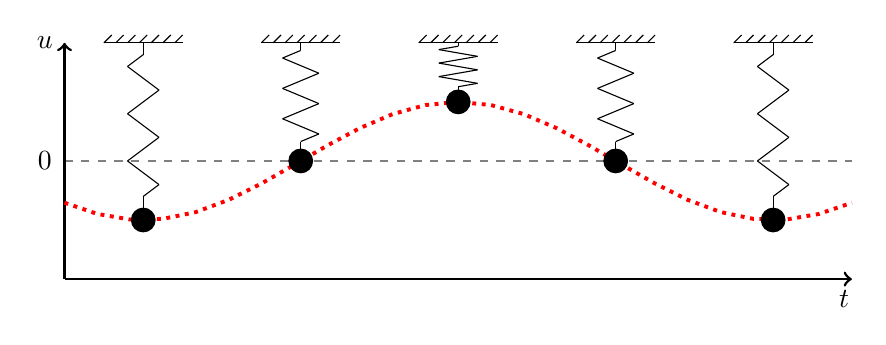
\begin{tikzpicture}
        
        \def\axisLineWidth{0.07};
            
        \def\zigzagLength{0.5}
        \def\zigzags{4}
        \pgfmathsetmacro\halfZigzags{\zigzags/2}
        \def\massSize{0.15}
        \def\massDistanceScaling{2}
        \def\amplitude{0.75}
        
        % axes
        \def\axisOffset{1}
        \draw[dashed, color = gray] (-\axisOffset, 0) -- (4*\massDistanceScaling+\axisOffset, 0);
        \node at (-\axisOffset-0.25, 1.5) {$u$};
        
        %u-axis
        \draw[->, line width=1] (-\axisOffset, -1.5) -- (-\axisOffset, 1.5);

        \node at (-\axisOffset - 0.25, 0) {$0$};

        %t-axis
        \draw[->, line width=1] (-\axisOffset, -1.5) -- (4*\massDistanceScaling+\axisOffset, -1.5);
        
        \node at (4*\massDistanceScaling + \axisOffset-0.1, -1.75) {$t$};

        % sine wave
        \draw[xshift=0 cm, xscale=4, domain=-0.25:2.25, dotted, variable=\x, red, line width=0.05cm] plot ({\x}, {-\amplitude*cos(180*\x)});

        \def\wallHeight{1.5}
        \def\wallHalf{0.5};
        \def\wallLineSpacing{0.15}
        \pgfmathsetmacro\halfNumDiag{\wallHalf / \wallLineSpacing}
        
        \foreach \massNo in {0, ..., 4}
        {
            \def\xshift{\massNo * \massDistanceScaling}

            \begin{scope}[xshift=\xshift cm]
                % draw wall
                \draw[-] (-\wallHalf, \wallHeight) -- (\wallHalf, \wallHeight) node[below, midway] (top) {};
                \foreach \bowDiag in {-\halfNumDiag, ...,\halfNumDiag}
                {
                    \draw[-] (\bowDiag * \wallLineSpacing, \wallHeight) -- (\bowDiag * \wallLineSpacing + 0.1, \wallHeight + 0.1);
                }
                
                \begin{scope}[yshift=1.5cm, rotate=180]
                    %spring extension
                    \pgfmathsetmacro\springHeight{1.5 + \amplitude*cos(\massNo * 90)}
    ;    
                    %what is the step in y
                    \pgfmathsetmacro\yInc{
                        (\springHeight-\massSize)/(2*(\zigzags+1)+4)
                    }

                    %what is the width of the spring based on its extension
                    \pgfmathsetmacro\halfSpringWidth{
                        0.5 * sqrt(\zigzagLength * \zigzagLength - 4 * \yInc * \yInc)
                    }

                    %small dot
                    \filldraw[black] (0, 0) circle (0pt) node[anchor=center](bottomSpring){};    

                    %start of spring
                    \draw[-] (0, 0) -- (0, \yInc);
                    \draw[-] (0, \yInc) -- (\halfSpringWidth, 2*\yInc);

                    % main zig zag
                    \def\curY{2*\yInc};
                    \def\curX{\halfSpringWidth};

                    \foreach \zig in {0, ...,\zigzags}
                    {
                        \pgfmathsetmacro\yToGoTo{\curY+2*\yInc};
                        % \filldraw[black] (0, \yToGoTo) circle (1pt) node[anchor=center](topSpring){\curX};           
                        \draw[-] (\curX, \curY) -- (-\curX, \yToGoTo);
                        \pgfmathsetmacro\tmpX{-\curX};

                        \global\let\curX=\tmpX;
                        \global\let\curY=\yToGoTo;
                    }

                    %end of spring
                    \pgfmathsetmacro\yToGoTo{\curY+\yInc};
                    \draw[-] (\curX, \curY) -- (0, \yToGoTo);
                    \global\let\curY=\yToGoTo;
                    \pgfmathsetmacro\yToGoTo{\curY+\yInc};
                    \draw[-] (0, \curY) -- (0, \yToGoTo);

                    %mass
                    \filldraw[black] (0, \yToGoTo+\massSize) circle (\massSize) node[anchor=center](topSpring){};   
                \end{scope}
            \end{scope}
        }
        % \node at (-0.5, 0.75) (K) {$K$};

    \end{tikzpicture}
    \caption{Mass spring system over time. The system follows a harmonic (sinusoidal) motion. \label{fig:massSpring}}
    \label{fig:lipSystem}
\end{figure}

\subsubsection{Intuition}
The behaviour of the mass-spring system in Eq. \eqref{eq:massSpringPDE} arises from two basic laws of physics: \textit{Newton's second law} and \textit{Hooke's law}. 

Starting with Newton's second law \textit{force equals mass times acceleration}, and relating this to the variables used in Eq. \eqref{eq:massSpringPDE} yields an expression for force
\begin{equation}\label{eq:newton2nd}
    F = M\ddot u.
\end{equation}
This equation in isolation can be used to, fx., calculate the force necessary to accelerate a mass of $M$ kg to $\ddot u$ m/s$^2$. Next, the force generated by the spring follows Hooke's law:
\begin{equation}\label{eq:hookesLaw}
    F = -Ku,
\end{equation} 
which simply states that the force generated by a spring with stiffness $K$ is negatively proportional to the value of $u$. In other words, the further the spring is extended (from the equilibrium $u=0$), the more force will be generated in the opposite direction. Finally, as the sole force acting on the mass is the one generated by the spring, the two expressions for the force $F$ can be set equal to each other and yields the equation for the mass-spring system in \eqref{eq:massSpringPDE}. 

The sinusoidal behaviour of the mass-spring system, or a least the fact that the mass ``gets pulled back'' to the equilibrium, is apparent from the minus-sign in Eq. \eqref{eq:hookesLaw}. The frequency of the sinusoid, depends on the value of $K$ as the ``pull'' happens to a higher degree for a higher spring stiffness. 
That the frequency of the system is also dependent on the mass $M$ can be explained by the fact that a lighter object is more easily moved and vice versa, which is apparent from Eq. \eqref{eq:newton2nd}. In other words, the pull of the spring has a greater effect on the acceleration of a lighter object than a heavier one. 

%Both these parameters affect the frequency through the definition of $\omega_0$ in Eq. \eqref{eq:omega0MassSpring}.

%From the definition of $\omega_0$ in Eq. \eqref{eq:omega0MassSpring} one can observe that a smaller $M$ will cause a higher frequency explained by the fact that a smaller mass is more easily moved. Similarly, a higher spring constant $K$ will cause a higher frequency, as the force caused by Hooke's law ``pulls'' the mass back to the equilibrium to a higher degree.

Finally, if $u = 0$ there is no spring force present and the acceleration remains unchanged. If the mass is not in motion, this means that it remains stationary, but if it is, the velocity is unchanged and it will continue moving with the same speed. 

\subsection{Discrete-time}
The displacement of the mass is approximated using 
\begin{equation}
    u(t) \approx u^n,
\end{equation}
with time $t = nk$, time step $k = 1/\fs$, sample rate $\fs$ and temporal index and $n \in \mathbb{N}^0$. Note that the ``grid function'' does not have a subscript $l$ as $u$ is not distributed in space and is now simply called a \textit{time series}.

Using the operators found in Section 
\ref{sec:FDoperators}, Eq. \eqref{eq:massSpringPDE} can be discretised as follows:
\begin{equation}\label{eq:massSpringFDS}
    M \dtt \un = -K\un,
\end{equation}
which is the first appearance of a FD scheme in this work. Expanding the $\delta_{tt}$ operator yields 
\begin{equation*}
    \frac{M}{k^2}\left(u^{n+1}-2\un+u^{n-1}\right) = -K\un,\nonumber
\end{equation*}
and solving for $u^{n+1}$ results in the following recursion or \textit{update equation}:
\begin{equation}\label{eq:massSpringUpdate}
    u^{n+1} = \left(2-\frac{Kk^2}{M} \right)\un - u^{n-1},
\end{equation}
which can be implemented in a programming language such as \texttt{MATLAB}. 

\subsection{Implementation and Output}
A simple \texttt{MATLAB} script implementing the mass-spring system described in this section is shown in Appendix \ref{app:massSpringCode}. The most important part of the algorithm happens in a for loop recursion, where update equation \eqref{eq:massSpringUpdate} is implemented. At the end of each loop, the system states are updated and prepared for the next iteration. %See Algorithm \ref{alg:massSpringLoop}

To be able to calculate the scheme at $n=0$ (the first time index of the simulation), values must be provided for $u^0$ and $u^{-1}$. These are determined by the initial conditions mentioned in Section \ref{sec:massSpringCont}. A simple way to obtain a sinusoidal motion with an amplitude of $1$, is to set the initial conditions as follows (using the backwards time difference operator for discretising the first-order time derivative): 
%
\begin{equation}
    u^0 = 1 \quad \text{and} \quad \dtm u^n = 0.
\end{equation}
The latter equality can be solved for $u^{-1}$ to obtain its definition: 
\begin{align*}
    &\frac{1}{k}\left(u^0 - u^{-1}\right) = 0,\\[-1em]
    \xLeftrightarrow{\mystrut\ u^0 = 1\ }\quad &1 - u^{-1} = 0,\\[0.1em]
 &u^{-1} = 1.
\end{align*}
To sum up, simply setting $u^0 = u^{-1} \neq 0$ \todo{maybe a bit short...} yields an oscillatory behaviour. 

The values for $K$ and $M$ are restricted by a stability condition which will be elaborated on in Section \ref{sec:stabilityAnalysis}.

The output of the system can be obtained by listening to the displacement of the mass at the given sample rate $\fs$. An example of this can be found in Figure \ref{fig:massSpringOutput} where the frequency of oscillation $f_0 = 440$ Hz.

\begin{figure}[ht]
    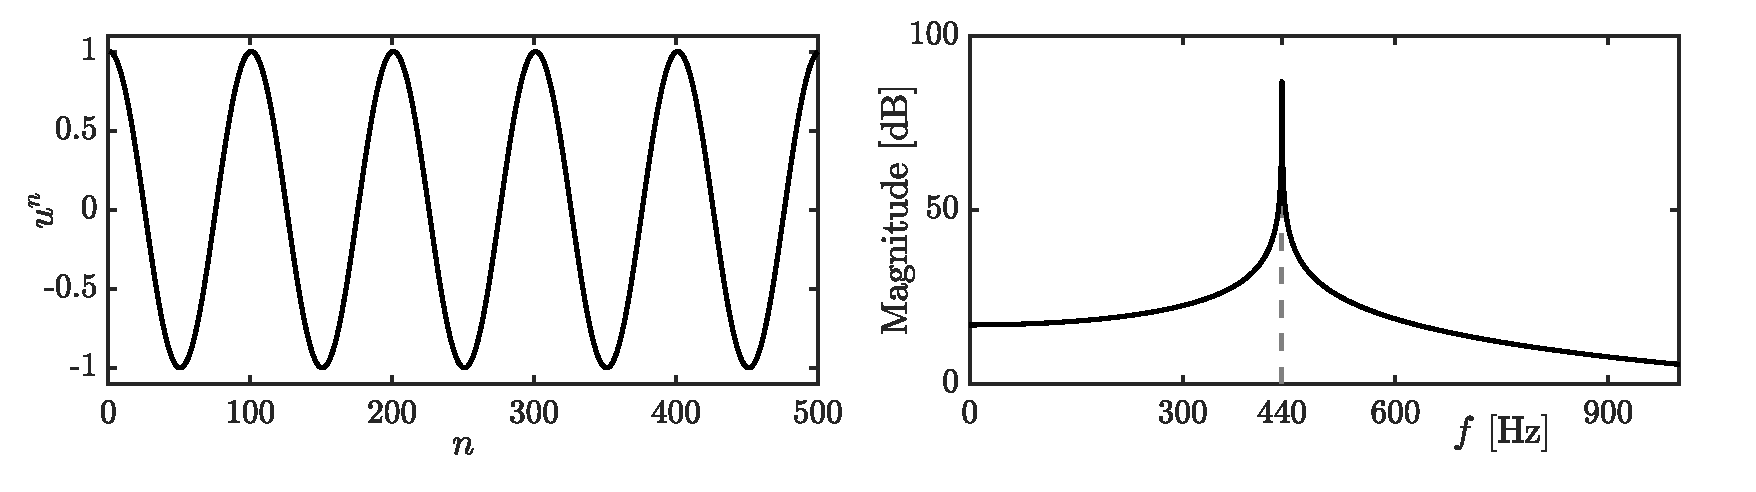
\includegraphics[width=\textwidth]{figures/fdtd/massSpringOutput.eps}
    \caption{The time-domain and frequency-domain output of a mass-spring system with $f_0 = 440$ Hz. \label{fig:massSpringOutput}}
\end{figure}


% \setlstMAT
% \begin{lstlisting}[caption=\texttt{MATLAB} implementation of a simple mass spring system. The code only shows the for-loop. The full code can be found in Appendix \ref{app:massSpringCode}., label=alg:massSpringLoop]
% %%% ... initialisation ... %%%

% %% Simulation loop
% for n = 1:lengthSound
    
%     % Update equation Eq. %*\eqrefMatlab[eq:massSpringUpdate] *)
%     uNext = (2 - K * k^2 / M) * u - uPrev; 
    
%     out(n) = u;
    
%     % Update system states
%     uPrev = u;
%     u = uNext;
% end
% \end{lstlisting}

\section{%Intro to PDEs: 
The 1D Wave Equation}\label{sec:1DWave}
Arguably the most important PDE in the field of physical modelling for sound synthesis is the 1D wave equation. It can be used to describe transverse vibration in an ideal string, longitudinal vibration in an ideal bar or the pressure in an acoustic tube (see Chapter \ref{ch:brass}). Although the behaviour of this equation alone does not appear in the real world \SWcomment[as such] -- as no physical system is ideal -- it is extremely useful as a test case and a basis for more complicated models. %Here, it will be used to introduce various concepts and analysis techniques in the field of FDTD methods.

\subsection{Continuous time\todo{FULL DOC SWEEP: check hyphen in titles}}
The 1D wave equation is a PDE that describes the motion of a system distributed in one dimension of space. Consider the state of a 1D system $u=u(x,t)$ of length $L$ defined for time $t\geq 0$ and $x\in \D$ with $D = [0, L]$. The PDE describing its motion is
\begin{equation}\label{eq:1DwavePDE}
    \ptt u = c^2 \pxx u,
\end{equation}
where $c$ is the wave speed (in m/s). 

\subsubsection{Intuition}
% Although the 1D wave equation often appears in the literature, an intuition or interpretation of why it works the way it does is hard to find. In the following, $u$ describes the transverse displacement of an ideal string.

% OR 

% I would like to use this opportunity to provide some extra explanation as to how and why the 1D wave equation in \eqref{eq:1DwavePDE} works the way it does. This will hopefully provide some basic intuition into the workings of PDEs that will make it easier to work with later on. \SWcomment[somethingsomething]

As with the mass-spring system in Section \ref{sec:massSpringSystem} the working of the PDE in \eqref{eq:1DwavePDE} arises from Newton's second law, even though this connection might be less apparent. %As in the mass-spring case, the acceleration of a system state is calculated, but now this depends on 

The 1D wave equation in \eqref{eq:1DwavePDE} states that the acceleration of $u = u(x,t)$ at location $x$ is determined by the second-order spatial derivative of $u$ at that same location (scaled by a constant $c^2$). In the case that $u$ describes the transverse displacement of an ideal string, this second-order derivative denotes the \textit{curvature} of this string. As $c^2$ is always positive, the sign (or direction) of the acceleration is fully determined by the sign of the curvature. In other words, a `positive' curvature at location $x$ along the ideal string yields a `positive' or upwards acceleration at that same location. 

What a `positive' or `negative' curvature implies is more easily seen when we take a simple function describing a parabola, $y(x) = x^2$, and take its second derivative to get $y''(x) = 2$. The answer is a positive number which means that $y$ has a positive curvature. 

So, what does this mean for the 1D wave equation? As a positive curvature implies a positive or upwards acceleration as per Eq. \eqref{eq:1DwavePDE}, $u$ with a positive curvature at a location $x$ will start to move upwards and vice versa. Of course, the state of a physical system such as $u$ will rarely have a perfect parabolic shape, but the argument still applies. See Figure \ref{fig:curvature}.

\begin{figure}[h]
    \centering
    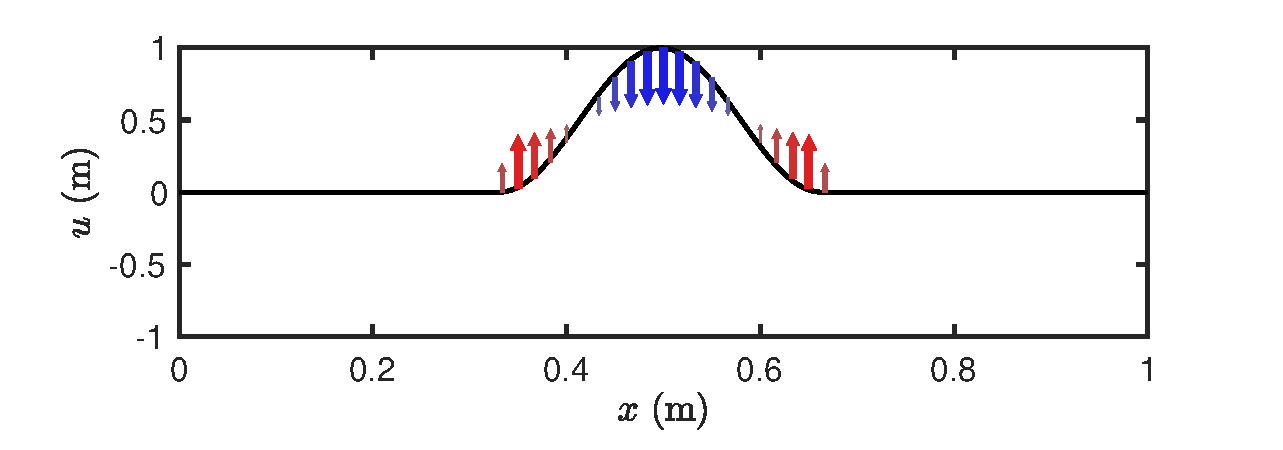
\includegraphics[width=\textwidth]{figures/resonators/curvature.eps}
    \caption{\label{fig:curvature} The forces acting on the 1D wave equation due to curvature. The arrows indicate the direction and magnitude of the force, and simultaneously the acceleration as these are connected through Eq. \eqref{eq:1DwavePDE}.}
\end{figure}\todo{different wording in caption}

\subsubsection{Boundary Conditions}
When a system is distributed in space, \textit{boundary conditions} must be determined.
Consider a system  of length $L$ (in m) defined over space $x\in \D$ where domain $\D = [0, L]$. Two often-used alternatives are
%
\begin{subequations}\label{eq:boundaryCond1DWave}
    \begin{align}
        u(0, t) = u(L, t) &= 0\quad \text{(Dirichlet, fixed)},\label{eq:contDirichlet}\\
        \px u(0, t) = \px u(L, t) &= 0\quad \text{(Neumann, free)}.\label{eq:contNeumann}
    \end{align}
\end{subequations}
%
The Dirichlet boundary condition says that at the end points of the system, the state is 0 at all times. The Neumann condition on the other hand, says that rather the slope of these points needs to be 0, but that the end points are free to move transversely. In the former case, incoming waves to invert after reaching the boundary whereas in the latter incoming waves are reflected un-inverted. See Figure \ref{fig:boundaryCondsCont}.

If both boundaries of the 1D wave equation share the same condition, the fundamental frequency of the simulation can be calculated using 
\begin{equation}\label{eq:fundamentalFreq}
    f_0 = \frac{c}{2L}\ .
\end{equation}

\begin{figure}[t]
    \centering
    \subfloat[The Dirichlet boundary condition in Eq. \eqref{eq:contDirichlet} fixes the boundary, which causes the incoming waves to invert.\label{fig:dirichlet}]{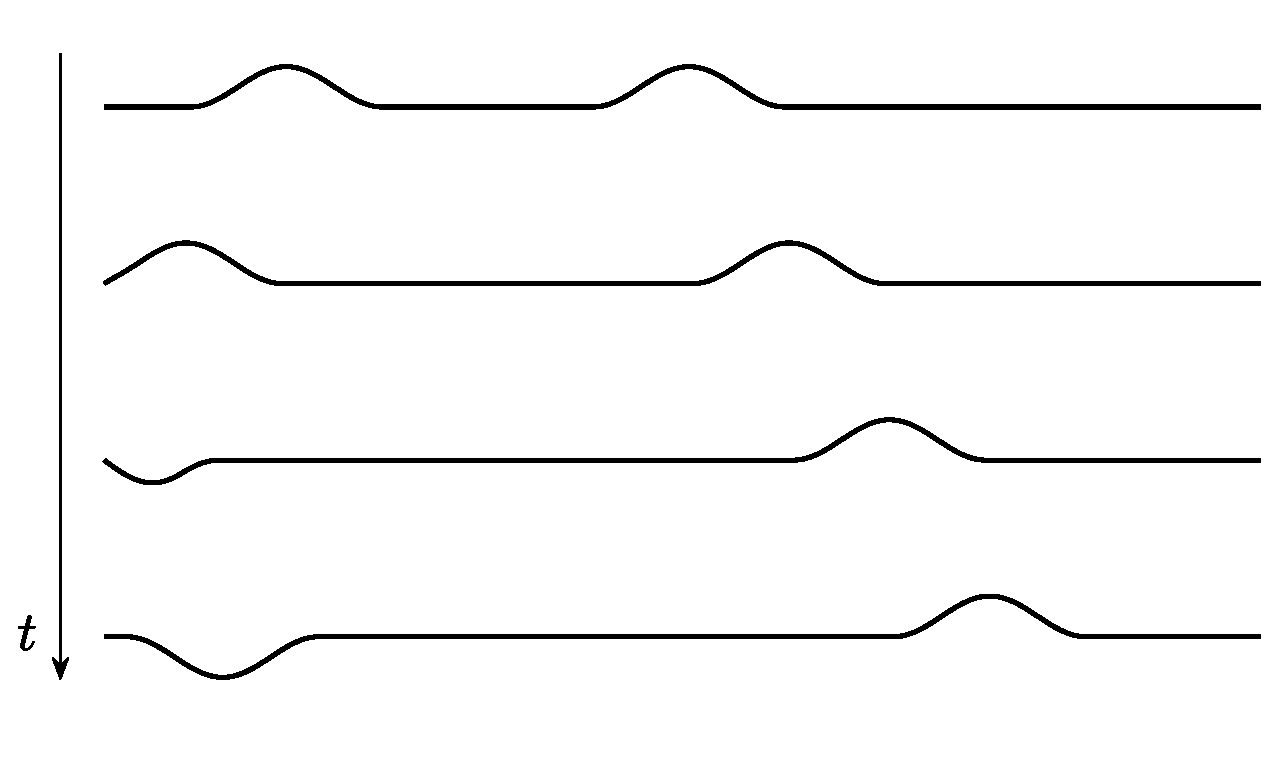
\includegraphics[width=0.45\textwidth]{figures/fdtd/dirichletCont.eps}}\hspace{0.06\textwidth}
    \subfloat[The Neumann or free boundary condition in Eq. \eqref{eq:contNeumann} fixes the slope at the boundary, causing the incoming waves to not invert.\label{fig:neumann}]{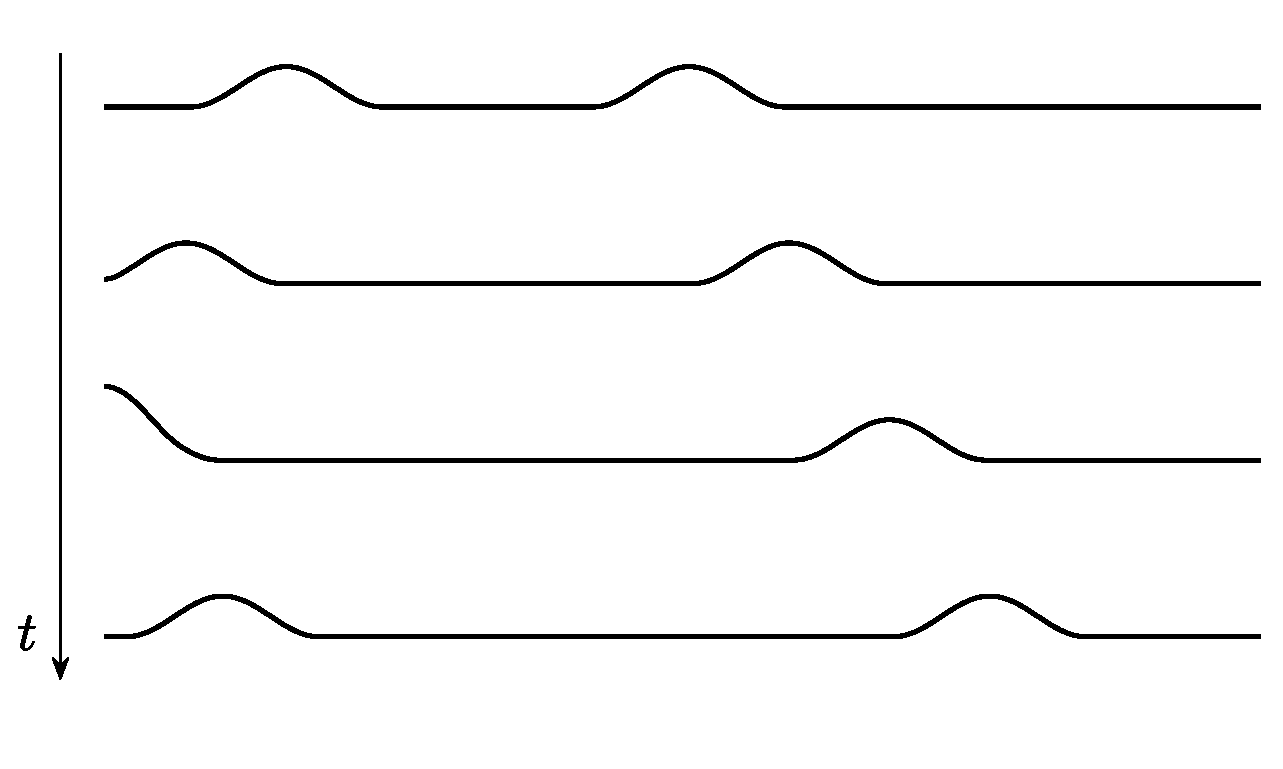
\includegraphics[width=0.45\textwidth]{figures/fdtd/neumannCont.eps}}
    \caption{The behaviour of the 1D wave equation with (a) Dirichlet or (b) Neumann boundary conditions.\label{fig:boundaryCondsCont}}
\end{figure}

\subsubsection{Scaling}
As this work follows much of Bilbao's \textit{Numerical Sound Synthesis} \cite{theBible}, it might be good to talk about a major discrepancy between the PDEs and FD schemes that appear there and those used here. Non-dimensionalisation, or \textit{scaling}, is extensively used in \cite{theBible} and much of the literature published around that time (fx. \cite{Bilbao2009,Bilbao2009spring}) and can be useful to reduce the amount of parameters used to describe a system.

Scaling techniques normalise the domain $x\in[0, L]$ to $x' = x/L$ such that $x' \in [0, 1]$. The 1D wave equation in \eqref{eq:1DwavePDE} can then be rewritten to
\begin{equation}\label{eq:scaled1Dwave}
    \ptt u = \gamma^2\partial_{x'x'}u,
\end{equation}
where scaled wave speed $\gamma = c/L$ has units of frequency. The scaling has removed the necessity for both $c$ and $L$ and simply specifying the scaled wave speed $\gamma$ is enough to parameterise the behaviour of the system. The parameter reduction gets more apparent for more complex systems and could greatly simplify of the models used, at least in notation and parameter control. 

Although this parameter reduction might be useful for resonators in isolation, when multiple resonators interact with each other (see Part \ref{part:interactions}), it is better to keep the systems dimensional. As a big part of this work includes interaction between multiple resonators, only dimensional systems will appear here.\todo{check whether still correct}

\subsection{Discrete time}
The most straightforward discretisation of Eq. \eqref{eq:1DwavePDE} is the following FD scheme
\begin{equation}\label{eq:1DwaveFDS}
    \dtt \uln = c^2 \dxx \uln,
\end{equation}
with $l\in\{0, \hdots, N\}$ and number of grid points $N + 1$.
Other schemes exist (see fx. \cite{theBible}), but are excluded as they have not been used in this work. Expanding the operators yields
\begin{equation}
    \frac{1}{k^2}\left(u_l^{n+1}-2 \uln + u_l^{n-1}\right) = \frac{c^2}{h^2} \left(u_{l+1}^n - 2 \uln + u_{l-1}^n\right).
\end{equation}
and solving for $u_l^{n+1}$ yields
\begin{equation}\label{eq:1DwaveUpdate}
    u_l^{n+1} = \left(2-2\lambda^2\right) \uln  + \lambda^2\left(u_{l+1}^n + u_{l-1}^n\right) - u_l^{n-1}.
\end{equation}
Here, 
\begin{equation}
    \lambda = \frac{ck}{h}
\end{equation}
is called the \textit{Courant number} and plays a big role in stability quality of the FD scheme. The Courant number needs to abide the (famous) Courant-Friedrichs-Lewy or \textit{CFL condition} for short \cite{Courant1928}
\begin{equation}\label{eq:CFL}
    \lambda \leq 1,
\end{equation}
which acts as a stability condition for scheme \eqref{eq:1DwaveFDS}.
If $\lambda = 1$, Eq. \eqref{eq:1DwaveFDS} is an exact solution to Eq. \eqref{eq:1DwavePDE}. \SWcomment[Exact solutions are actually quite uncommon in the realm of differential equations!] If $\lambda < 1$, the quality of the simulation quality decreases and dispersive and bandlimiting effects occur (see Section \ref{sec:output1DWave}).

\subsubsection{Stencil}
It can be useful to visualise the \textit{stencil}, or region of operation, of a FD scheme. A stencil visualises what grid values are necessary to calculate the state at the next time step $u_l^{n+1}$. Figure \ref{fig:stencil1DWave} shows the stencil for scheme \eqref{eq:1DwaveFDS} and in essence visualise the various appearances of the grid function in \eqref{eq:1DwaveUpdate}. 

\begin{figure}[h]
    \centering
    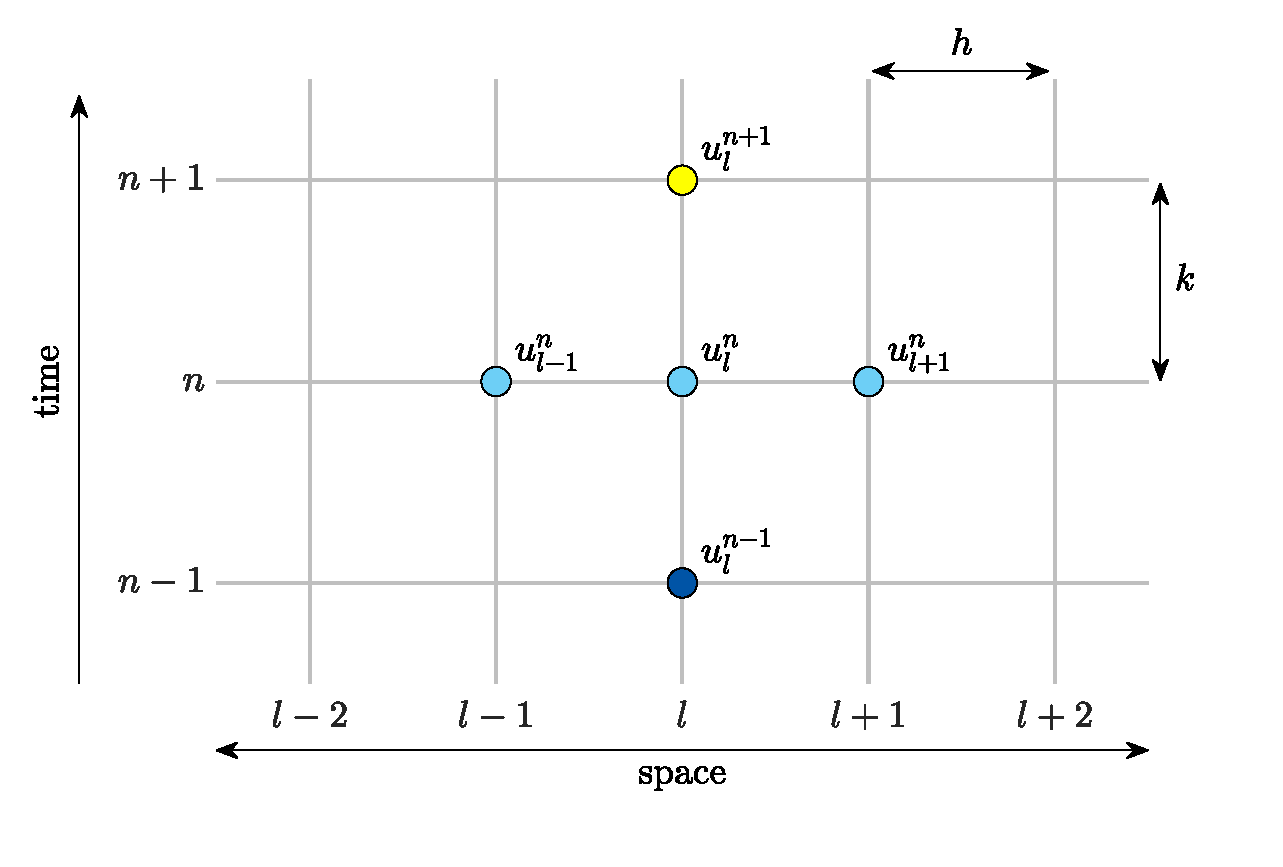
\includegraphics[width=0.8\textwidth]{figures/fdtd/1DWaveStencil.eps}
    \caption{The stencil, or region of operation, for the FD scheme in \eqref{eq:1DwaveFDS}.\label{fig:stencil1DWave}}
\end{figure}

\subsubsection{Boundary Conditions}
The end points of the discrete domain are located at $l = 0$ and $l = N$.
Substituting these locations into Eq. \eqref{eq:1DwaveUpdate} seemingly shows that grid points outside of the defined domain are needed, namely $u_{-1}^n$ and $u_{N+1}^n$. These can be referred to as \textit{virtual grid points} and can be accounted for %/defined
by discretising the boundary conditions in Eq. \eqref{eq:boundaryCond1DWave}. Discretising these (using the centred spatial difference operator for the Neumann condition) yields
\begin{subequations}
    \begin{align}
        u_0^n = u_N^n &= 0, \quad\text{(Dirichlet)}\label{eq:discreteDirichlet}\\
        \delta_{x\cdot} u_0^n = \delta_{x\cdot} u_N^n &= 0. \quad \text{(Neumann)}\label{eq:discreteNeumann}
    \end{align}
\end{subequations}
Expanding the operators in Eq. \eqref{eq:discreteNeumann} and solving for $u_{-1}^n$ and $u_{N+1}^n$ provides the definitions for these virtual grid points based on values in the discrete domain:

\begin{minipage}[c]{0.49\textwidth}
    \begin{align*}
        &\frac{1}{2h} \left(u_1^n - u_{-1}^n\right) = 0,\\
        &u_1^n - u_{-1}^n = 0,\\
        &u_{-1}^n = u_1^n.
    \end{align*}
\end{minipage}
\begin{minipage}[c]{0.49\textwidth}
    \begin{align*}
        &\frac{1}{2h} \left(u_{N+1}^n - u_{N-1}^n\right) = 0,\\
        &u_{N+1}^n - u_{N-1}^n = 0,\\
        &u_{N+1}^n = u_{N-1}^n.
    \end{align*}
\end{minipage}
\\

\noindent If Dirichlet boundary conditions are used, the states of the boundary points will always be zero and can therefore can be excluded from the calculations. The range of calculation then simply becomes $l\in\{1,\hdots, N-1\}$. If, on the other hand, Neumann conditions are used, the update equation in \eqref{eq:1DwaveUpdate} at the boundaries will have the the above definitions for the virtual grid points substituted at $l = 0$ and $l = N$ and will become 

\begin{equation}\label{eq:1DWaveLeftBound}
    u_0^{n+1} = \left(2-2\lambda^2\right) u_0^n  + 2\lambda^2 u_1^n - u_0^{n-1},
\end{equation}
and 
\begin{equation}\label{eq:1DWaveRightBound}
    u_N^{n+1} = \left(2-2\lambda^2\right) u_N^n  + 2\lambda^2 u_{N-1}^n - u_N^{n-1},
\end{equation}
at the left and right boundary respectively.

\subsection{Implementation and Output}\label{sec:output1DWave}
As $c$, $k$ and $h$ are interdependent due to the CFL condition in \eqref{eq:CFL}, it is useful to rewrite this condition in terms of known variables.
As the time step $k$ is based on the sample rate and thus (usually) fixed, and $c$ is a user-defined wave speed, Eq. \eqref{eq:CFL} can be rewritten in terms of the grid spacing $h$:
\begin{equation}\label{eq:1DWaveStabilityCond}
    h \geq ck,
\end{equation}
%
which, in implementation, is used as a stability condition for the scheme. See Section \ref{sec:stabilityAnalysis} for more information on how to derive the stability condition from a FD scheme.
Again, if Eq. \eqref{eq:1DWaveStabilityCond} is satisfied with equality, the FD scheme is an exact solution to the PDE, and if $h$ deviates from this condition, the quality of the simulation decreases. 

So why would the stability condition not be satisfied with equality? As mentioned in Section \ref{sec:gridFunctions}, a continuous domain $\D = [0,L]$ for a system of length $L$ needs to be divided into $N$ equal sections of length $h$. A logical step to calculate $N$ would be to divide $L$ by $h$ calculated using \eqref{eq:1DWaveStabilityCond} satisfied with equality. However, this calculation might not result in an integer value, which $N$ should be! To stay as close to the stability condition as possible, the following calculations are performed in order:
\begin{equation}\label{eq:orderOfCalc}
    h := ck, \quad N := \floor[\frac{L}{h}], \quad h := \frac{L}{N}, \quad \lambda := \frac{ck}{h},
\end{equation}
where $\floor[\cdot]$ denotes the flooring operation. In other words, Eq. \eqref{eq:1DWaveStabilityCond} is satisfied with equality and used to calculate integer $N$. After this, $h$ is recalculated based on $N$ and used to calculate the Courant number $\lambda$. This process assures that $N$ is an integer and that the CFL condition is satisfied, though not necessarily with equality.

If this recalculation of $h$ is not carried out, the behaviour of the system will not be correct. For example, we want our 1D wave equation to be 1 m long ($L = 1$) and produce a fundamental frequency of $f_0 = 750$ Hz according to \eqref{eq:fundamentalFreq}. This requires a wave speed of $c = 1500$ m/s. If we use a commonly-used sample rate of $\fs = 44100$ Hz, and recalling that $k = 1/\fs$, these values can be filled into \eqref{eq:1DWaveStabilityCond} satisfied with equality yielding $h \approx 0.034$. If we divide the length by the grid spacing, we get $L / h = 29.4$, meaning that exactly $29.4$ intervals of size $h$ fit in the domain $\D$. However, the number of intervals needs to be an integer and -- using the above values -- we get $N = 29$. If $h$ is not recalculated according to \eqref{eq:orderOfCalc}, the total length will be $29$ times the grid spacing $h$. This results in $L \approx 0.986$ and is slightly less than the original length of $1$. Although the CFL condition will be satisfied with equality, the fundamental frequency will be slightly tuned up: $f_0 \approx 760.34$ Hz. If $h$ is recalculated based on $N$, $L$ and $f_0$ will be unchanged, and $\lambda \approx 0.986$ which is still very close to satisfying condition \eqref{eq:CFL}.

% Together with the total length of the domain $L$, $h$ can be used to determine into how many intervals $N$ the continuous domain can be subdivided in . As this number is an integer,  This number of intervals $N$ and through that the Courant number $\lambda$ can be calculated using the following operations
% \begin{equation}
%     h := ck, \quad N := \floor[\frac{L}{h}], \quad h := \frac{L}{N} \quad \lambda := \frac{ck}{h}.
% \end{equation}
% where $\floor[\cdot]$ denotes the flooring operation and is necessary as $N$ is an integer. The CFL condition in Eq. \eqref{eq:CFL} thus places a limit on the grid spacing $h$ and with that the number of grid points allowed by the simulation.

\subsubsection{Output}
After the system is excited (see \ref{part:exciters}), one can retrieve the output of the system by selecting a grid point and listening to that at at the given sample rate $\fs$. The amount of modes is determined by the number of moving points in the system. If Dirichlet boundary conditions are used this means that there are $N-1$ modes, and $N+1$ modes for Neumann boundary conditions.

If the CFL condition is satisfied with equality, these modes are integer multiples of the fundamental: $f_m = mf_0$ for mode number $m \in \{1, \hdots, N-1\}$ for Dirichlet and $m \in \{0, \hdots, N\}$ for Neumann boundary conditions. The frequency of the harmonic partials can also be analytically / numerically derived using modal analysis as will be explained in Section \ref{sec:modalAnalysis}.

The amplitude of the different modes, on the other hand, depends on the location of excitation and output. 
\SWcomment[modes]


See Appendix \ref{app:1DWave}\texttt{MATLAB} implementation of the 1D wave equation

\def\figSpacing{0.01\textwidth}
\def\figWidth{0.32\textwidth}

\begin{figure}[t]
    \centering
    \subfloat[$\lambda = 1$\label{fig:1DWaveDisp1}]{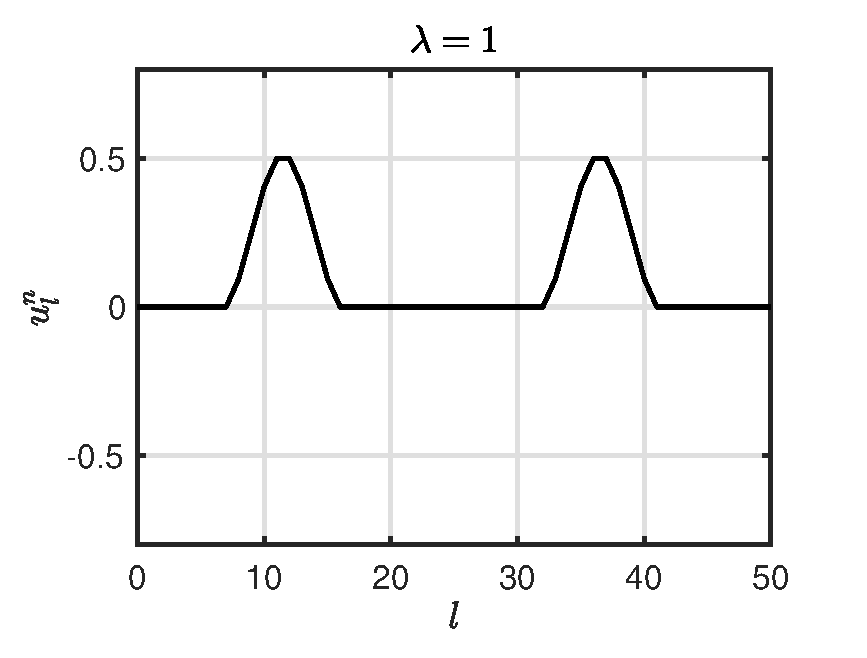
\includegraphics[width=\figWidth]{figures/fdtd/ulnLambda1.eps}}\hspace{\figSpacing}
    \subfloat[$\lambda = 0.9$ \label{fig:1DWaveDisp09}]{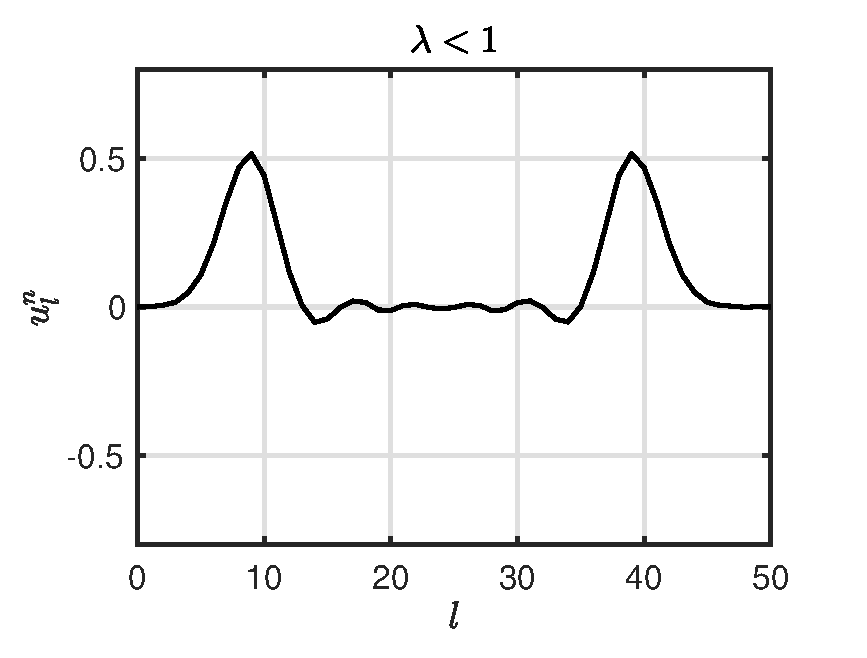
\includegraphics[width=\figWidth]{figures/fdtd/ulnLambda09.eps}}\hspace{\figSpacing}
    \subfloat[$\lambda = 1.001$\label{fig:1DWaveDisp1001}]{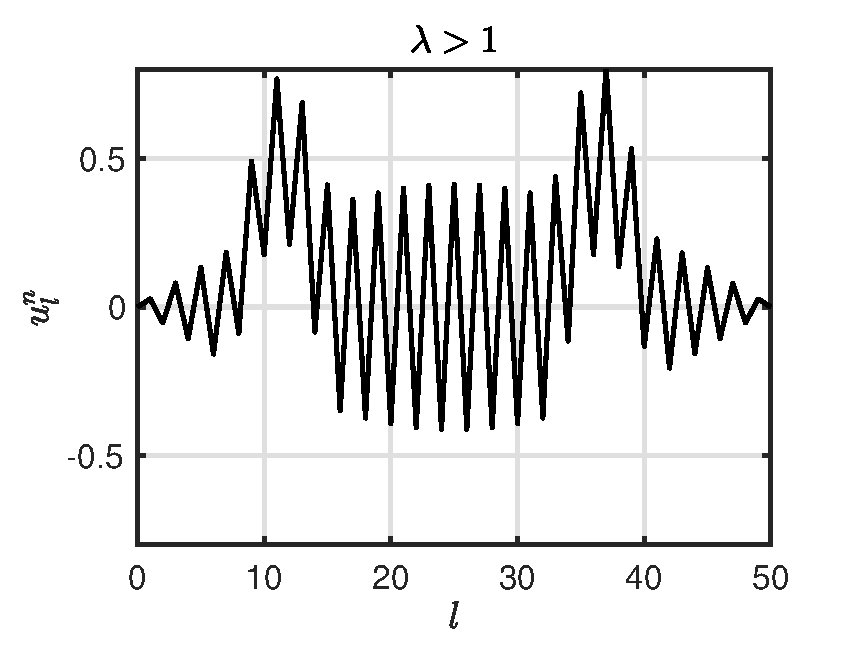
\includegraphics[width=\figWidth]{figures/fdtd/ulnLambda1001.eps}}
    \caption{State $\uln$ with $N = 50$ and $f_\text{s} = 44100$ visualised $\sim\!100$ samples after excitation. (a) If $\lambda = 1$, the solution is exact. (b) If $\lambda < 1$ dispersive behaviour shows. (c) If $\lambda > 1$ the CFL condition in Eq. \eqref{eq:CFL} is not satisfied and the system is unstable.\label{fig:1DWaveDispersion}\SWcomment[caption is straight from paper]}
\end{figure}

\begin{figure}[t]
    \centering
    \subfloat[$\lambda = 1$\label{fig:1DWaveBand1}]{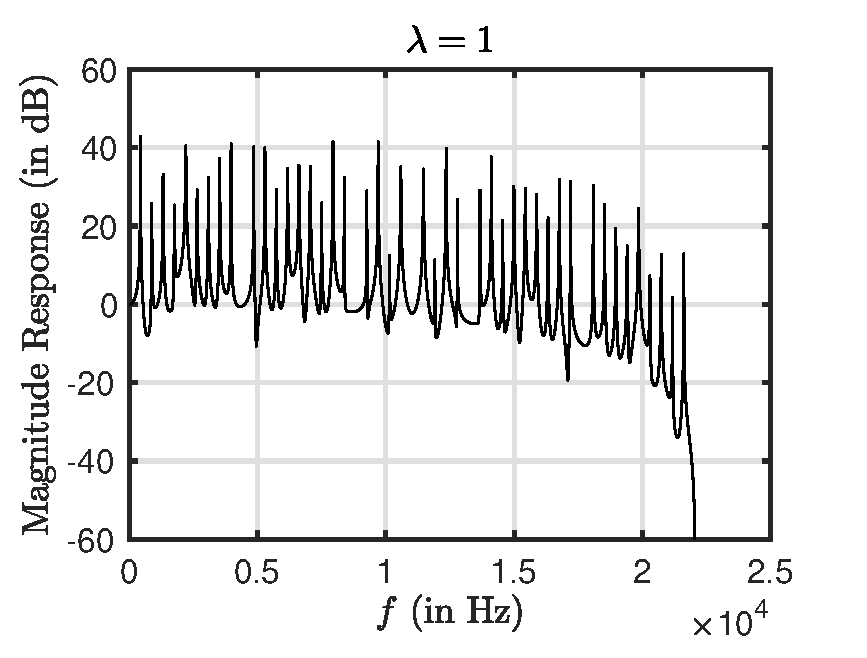
\includegraphics[width=\figWidth]{figures/fdtd/bandwidthLambda1.eps}}\hspace{\figSpacing}
    \subfloat[$\lambda = 0.9$ \label{fig:1DWaveBand09}]{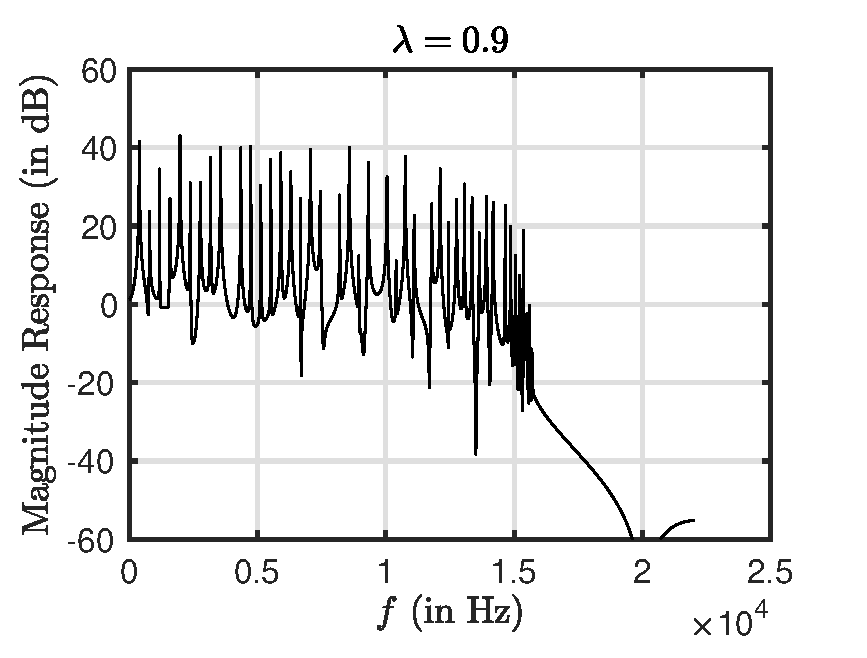
\includegraphics[width=\figWidth]{figures/fdtd/bandwidthLambda09.eps}}\hspace{\figSpacing}
    \subfloat[$\lambda = 1.001$\label{fig:1DWaveBand1001}]{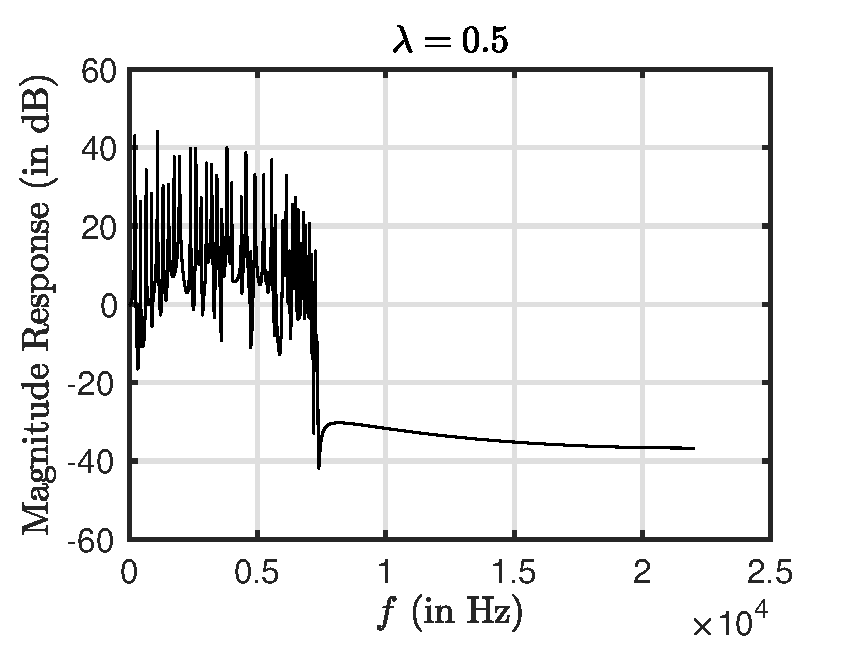
\includegraphics[width=\figWidth]{figures/fdtd/bandwidthLambda05.eps}}
    \caption{Bandwidths of the simulation output at $l = 16$ 
    with $f_\text{s} = 44100$ Hz and $N = 50$ excited with a raised cosine with a width of 5 at center-location $N = 25$. The Courant number is set to (a) $\lambda = 1$, (b) $\lambda = 0.9$ and (c) $\lambda = 0.5$.\label{fig:1DWaveBandwidth}\SWcomment[caption is straight from paper]}
\end{figure}